\documentclass[../main.tex]{subfiles}

\begin{document}
\section{파이썬의 특징}
파이썬은 1991년에 \alt*{귀도 반 로섬}{Guido van Rossum}이 발표한 프로그래밍 언어로, 문법이 굉장히 단순하면서 높은 생산성을 가지고 있는 언어입니다.\footnote{귀도 반 로섬은 1989년 크리스마스 연휴에 취미로 프로그래밍 언어를 만들었는데, 이것이 파이썬의 시초가 되었습니다.}
특히 파이썬으로 (잘) 작성된 코드는 \alt*{의사코드}{pseudocode}처럼 쉽게 읽히기 때문에 진입 장벽이 낮고 비교적 배우기가 쉽습니다.
이러한 특징 덕분에 많은 학교에서는 프로그래밍 입문 수업을 파이썬으로 진행하고 있습니다.\footnote{과거에 BASIC, C, 자바 등으로 교육을 한 학교들도 점차 파이썬으로 커리큘럼을 바꾸어 나가고 있는 추세입니다.}

하지만 뭐니뭐니해도 파이썬의 가장 큰 장점은, \emph{\alt*{파이썬 패키지 인덱스}{Python Package Index, PyPI}에 포함된 방대한 양의 패키지 생태계입니다.}
이 때문에 파이썬은 흔히 ``\alt*{배터리가 포함된}{batteries included}'' 언어라고 불립니다 (그림~\ref{fig:meme}).
따라서 파이썬을 사용하면 기존에 만들어진 도구들을 조립하여 원하는 프로그램을 빠르게 만들어낼 수 있습니다.

\begin{figure}[htbp]
  \centering
  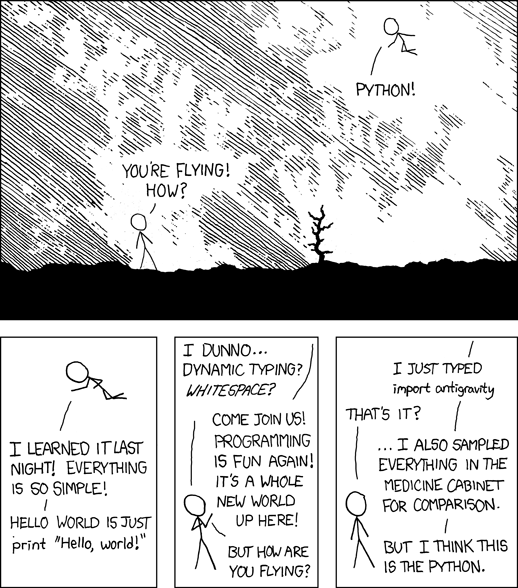
\includegraphics[width=0.7\linewidth]{./figures/xkcd_python}
  \caption{파이썬은 배터리가 포함된 언어입니다. 출처: \url{https://xkcd.com/353/}}\label{fig:meme}
\end{figure}

프로그래밍에 익숙하지 않은 사람도 컴퓨터에 관심이 있다면 C, C++, \alt*{자바}{Java} 등의 언어와 함께 파이썬도 한 번 쯤 들어보았을 정도로, 파이썬은 점유율 상위 다섯 언어 안에 드는 주류 언어입니다.
파이썬은 1995년에 등장한 자바보다도 오래 전에 만들어진 언어로, 짧지 않은 역사를 가지고 있습니다.\footnote{이 글을 작성하는 현 시점의 파이썬 최신 버전은 3.11.1입니다.}

파이썬은 \alt*{실행}<실행기>{inpterpreted}[interpret]<interpreter> 언어입니다.
실행 언어란 \alt*{실행기}{interpreter}가 코드를 한 줄씩 읽으면서 그때그때 ``동시 통역''하는 방식의 언어입니다.
이와 대조되는 방식은 \alt*{번역}{compiled}[compile]입니다.
번역 언어는 \alt*{번역기}{compiler}가 코드 전체를 먼저 기계어로 ``통번역''이 되어야 실행할 수 있습니다.
이때 기계어는 주어진 CPU와 \alt*{운영체제}{operating system, OS}가 바로 이해할 수 있는 형태의 저수준 언어입니다.
C와 같은 언어가 이에 해당됩니다.
이 때문에 번역 언어는 번역된 결과물의 실행 속도가 빠르다는 장점이 있지만, 프로그램을 수정하기 위해서 아무리 작은 변화를 주더라도 전체 코드를 다시 한 번 번역하는 과정이 필요합니다.\footnote{엄밀하게 말하면 언어 자체가 실행되는지 번역되는지를 결정하는 것이 아니라, 언어의 \alt*{구현}{implementation}이 실행기인지 번역기인지 나뉘게 됩니다. 주어진 언어에 대해서 여러 구현이 존재할 수 있기 때문입니다. 파이썬의 경우, CPython\index{CPython}은 실행기 방식으로 만들어져 있습니다.}

이제 파이썬이 얼마나 쉽고 직관적인 언어인지 알아봅시다.
아래는 \verb/A+/가 \verb/F/, \verb/C+/, \verb/B0/, \verb/A-/, \verb/A+/의 목록\index{\texttt{list}}에 포함\index{\texttt{in}}되어 있으면 \verb/A+가 있습니다./를 출력\index{\texttt{print}}하는 파이썬 코드입니다:
\begin{minted}{python}
if "A+" in ["F", "C+", "B0", "A-", "A+"]:
    print("A+가 있습니다.")
\end{minted}
프로그래밍을 할 줄 모르더라도 위 코드가 어떤 일을 하는지는 대강 이해할 수 있습니다.
사람이 구사하는 문장과 크게 다르지 않기 때문입니다.
이처럼 파이썬으로는 하고 싶은 일을 직관적으로 코드로 옮길 수 있습니다.

반면 C 언어에서는 위와 같은 작업을 하기 위해서 아래와 같은 코드를 작성해야 합니다:
\begin{minted}{c}
#include <stdio.h>
#include <string.h>
int main(int argc, char *argv[]) {
    char grades[][3] = {"F", "C+", "B0", "A-", "A+"};
    for (int i = 0; i < 5; ++i) {
        if (strncmp(grades[i], "A+", 2) == 0) {
            printf("A+가 있습니다.\n");
            break;
        }
    }
    return 0;
}
\end{minted}
단 두 줄의 파이썬 코드로 될 일을 C 언어로는 10줄 이상으로 작성해야 하는 것입니다.\footnote{이는 C가 나쁘다는 것을 보여주는 것이 아니라, 파이썬으로 얼마나 간결하고 빠르게 코드를 작성할 수 있는지를 보여주는 예시입니다. C는 시스템 수준의 작업을 할 때 꼭 필요한 매력적인 언어입니다.}

\section{파이썬의 기본 요소}
\subsection{안녕, 세상!}

\begin{figure}[htpb]
  \centering
  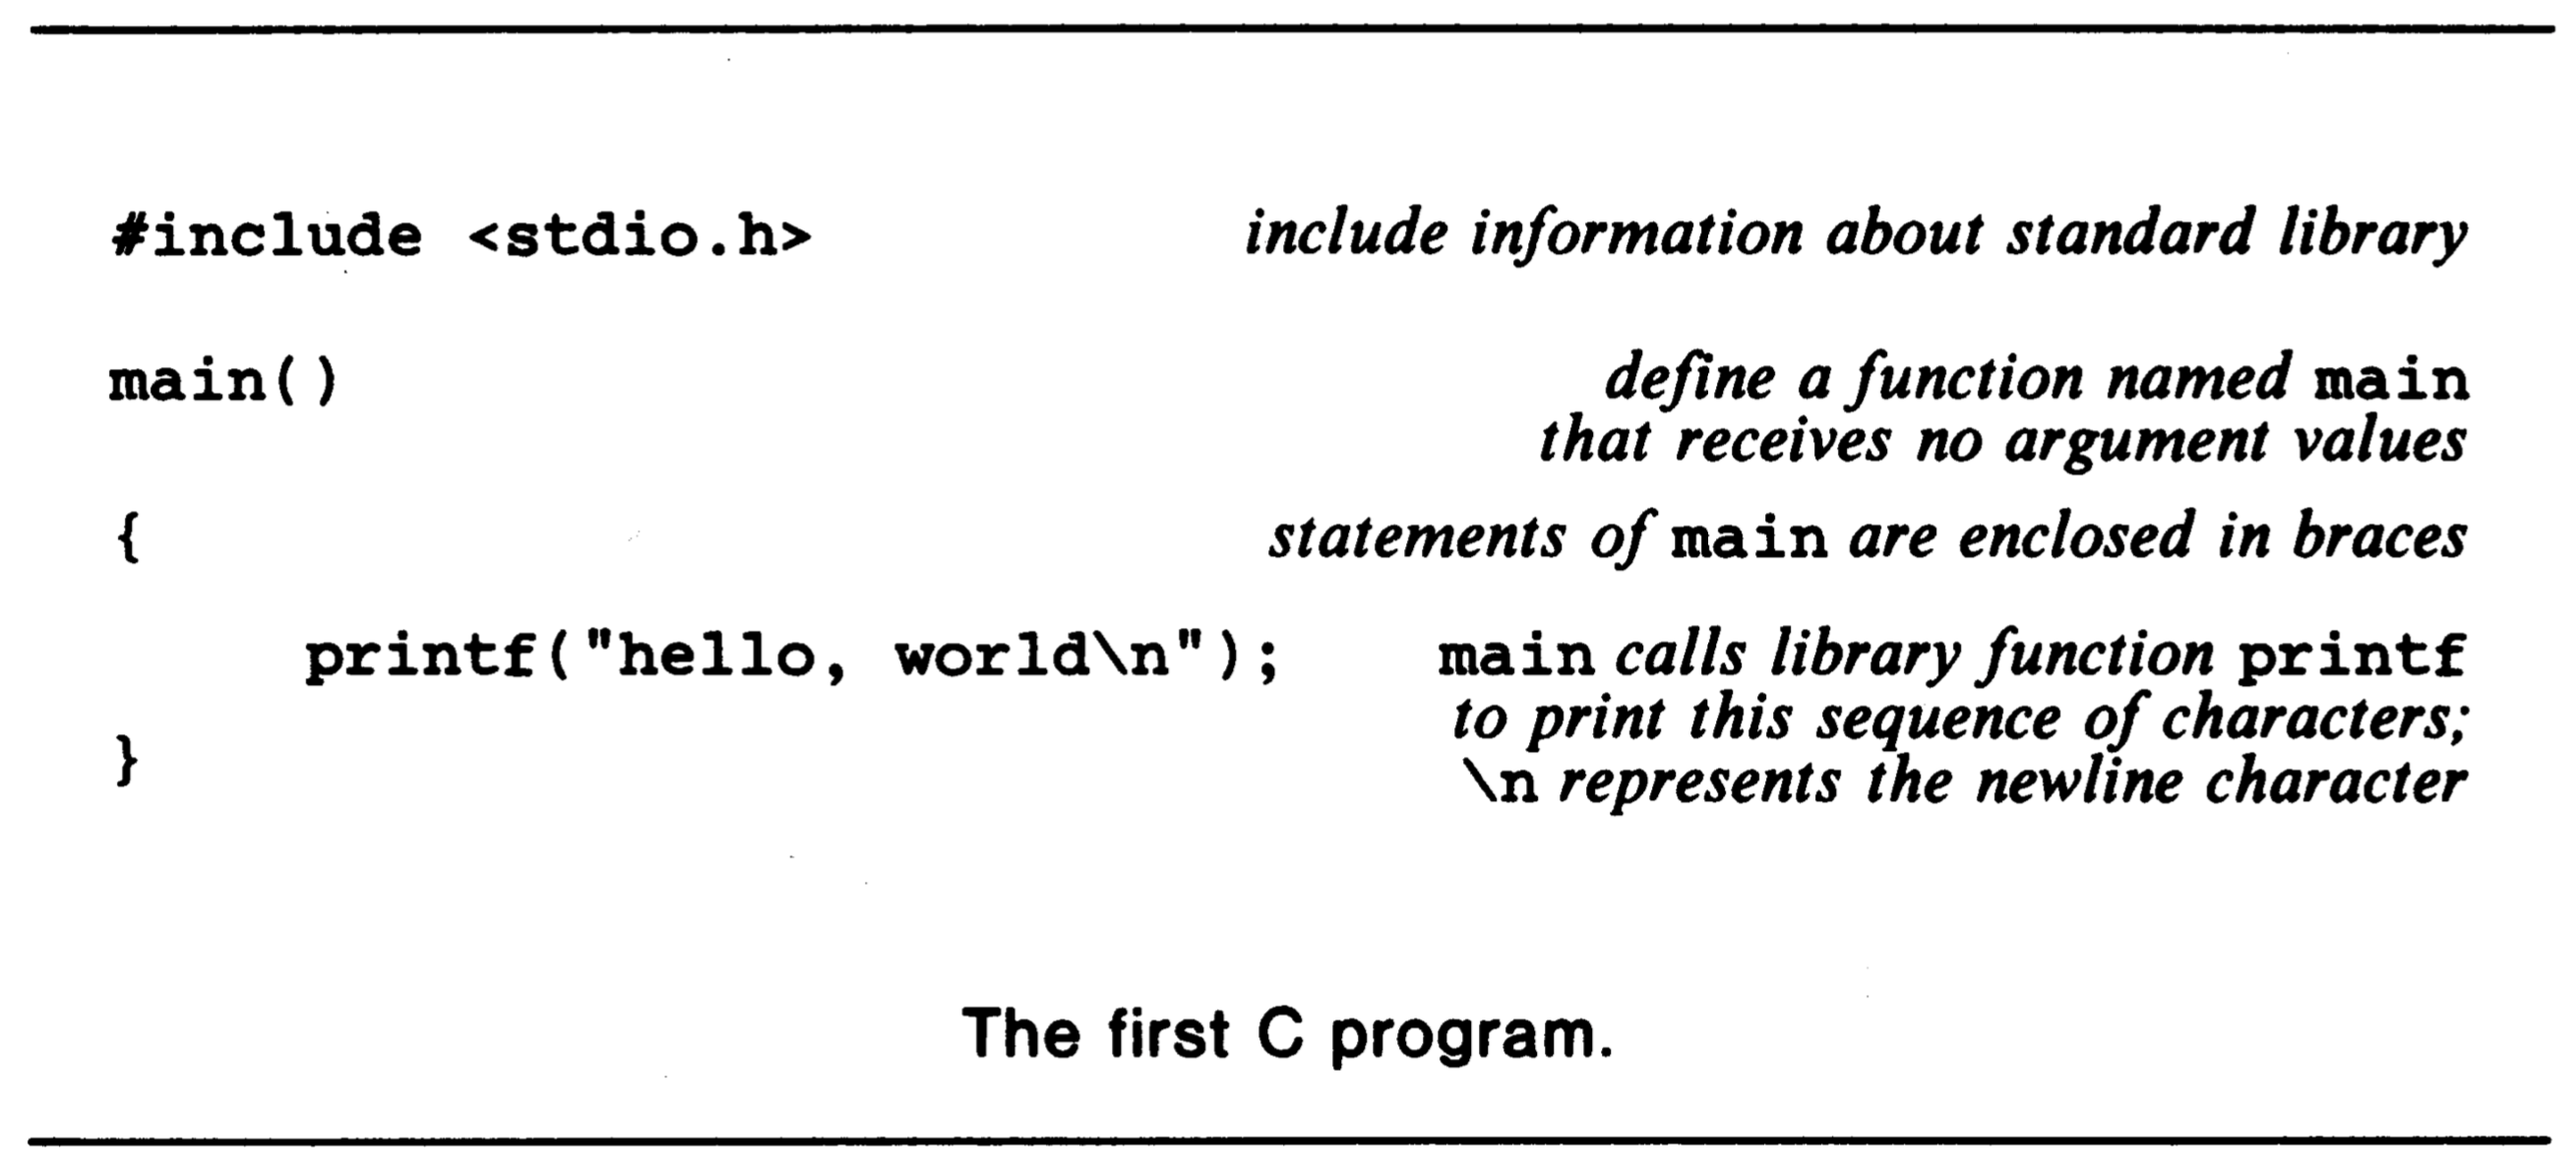
\includegraphics[width=0.8\linewidth]{./figures/hello_world.png}
  \caption{K\&R \booktitle{The C Programming Language}의 첫 프로그램}\label{fig:hello}
\end{figure}

1978년에 출판된 \booktitle{The C Programming Language}\footnote{저자인 Brian Kernighan\index{Brian Kernighan}과 Dennis Ritchie\index{Dennis Ritchie}의 초성을 딴 K\&R로 흔히 불리웁니다.}에서 예시로 사용된 이후 첫 프로그램은 보통 \texttt{Hello, World!}를 출력하는 것으로 시작됩니다 (그림~\ref{fig:hello}).
먼저, \alt*{통합 개발 환경}{integrated development environment, IDE}\footnote{PyCharm\index{PyCharm}, Wing IDE\index{Wing IDE} 등이 있습니다.}이나 \alt*{텍스트 편집기}{text editor}\footnote{Visual Studio Code\index{Visual Studio Code}, vi(m)\index{vi|seealso{vim, GNU Emacs}}\index{vim|see{vi}}, GNU Emacs\index{GNU Emacs}\index{Emacs|see{GNU Emacs}} 등이 있습니다. 저자는 vim을 8년 넘게 사용하다가 GNU Emacs로 이주하였습니다.}에 다음과 같은 코드를 입력해봅시다:
\begin{minted}{python}
print("Hello, World!")
\end{minted}
이를 실행하면 \verb/Hello, World!/가 출력될 것입니다.
이제 파이썬의 문법에 대해서 본격적으로 알아봅시다.

\subsection{값과 변수}
파이썬의 Integrated Development and Learning Environment, IDLE\index{Integrated Development and Learning Environment, IDLE}이나 \alt{쉘}{shell}에서 직접 파이썬 실행기를 실행하여 다음을 입력해 봅시다.\footnote{다시 언급하자면, 파이썬은 실행 언어이기 때문에 명령을 한 줄씩 입력하여 명령을 수행할 수 있는 것입니다.}
(\verb/>>>/는 직접 입력하는 것이 아니라 IDLE 혹은 쉘이 새로운 입력을 받기 위해 표시하는 것입니다.)
\begin{minted}{python}
>>> a = (1 + 2 + 3 + 4) // 2
>>> b = a - 1
>>> c = 3
>>> print(b + c)
7
>>> print(b, c)
4  3
>>> d = c
>>> a = d
>>> print(a)
3
\end{minted}
\pyin{a = (1 + 2 + 3 + 4) // 2}는 등호 왼쪽에 있는 \verb/a/에 등호 오른쪽에 있는 $\frac{1+2+3+4}{2}$를 계산한 결과를 \alt*{대입}{assign}\index{\texttt{=}|see{대입}}한다는 뜻입니다.
즉, 수학에서 말하는 등호와는 의미가 다른 것이지요.
줄 2의 \pyin{b = a - 1}은 현재 \verb/a/에 배정\myindex{배정}{assign}된 $\frac{1+2+3+4}{2} = 5$의 값에서 1을 뺀 4를 \verb/b/에 배정한다는 뜻입니다.
이 때 좌변에 있는 \verb/a/, \verb/b/, \verb/c/를 \alt*{변수}{variable}, 우변의 \pyin{(1 + 2 + 3 + 4) // 2}를 \alt*{식}{expression}이라고 합니다.
또한 이러한 변수에 배정되는 결과를 \alt*{값}{value}이라고 합니다.
다시 위의 예시로 돌아가서, 줄 2에 있는 좌변의 \verb/b/는 변수, 우변의 \pyin{a - 1}는 식, 그 결과인 \verb/4/는 값인 것이죠.
영어 문장으로 ``let \{variable\} be \{value\}.''가 말이 되는지 대입하여 보면 쉽게 알 수 있습니다.

변수와 값은 문자인지 숫자인지의 여부가 아니라 대입이 되는 대상인지 대입이 되어지는 대상인지의 여부가 결정짓습니다.\footnote{실제로 이렇게 간단하지는 않지만, 지금의 시점에서는 이렇게 이해하셔도 좋습니다.}
식의 구성 요소가 변수 하나만 있는 경우, 그 ``결과''는 값이 될 수 있습니다.
줄 8의 같은 경우, 우변의 \verb/c/는 변수이고, \verb/d/라는 변수에 대입될 값을 만드는 식입니다.

그렇다면, 다음과 같은 표현을 어떨까요?
\begin{minted}{python}
>>> 10 = a
\end{minted}
지금까지 잘 따라왔다면, 변수가 위치해야 할 좌변에 값인 \alt*{리터럴}{literal}\footnote{\texttt{0}은 \alt*{정수}{integer} 리터럴, \texttt{"python"}은 \alt*{문자열}{string} 리터럴입니다. 정수와 문자열은 (뒤에 알아볼) \alt*{타입}{type}입니다.}이 위치한 잘못된 표현인 것을 알 수 있습니다.
실제로 이를 실행하면 \texttt{SyntaxError: cannot assign to literal here. Maybe you meant '==' instead of '='?}와 같은 문구를 확인할 수 있습니다.
이처럼 파이썬은 우리가 잘못된 표현을 실행하려고 하면 최대한 그 잘못을 알려주려고 합니다.
따라서 앞으로 이와 같은 에러를 마주치면 반드시 뭐라고 써있는지 꼼꼼히 확인하는 습관을 들여야 합니다.

값은 여러 종류로 분류할 수 있습니다.
이러한 분류 기준을 \alt*{자료형}<타입>{data type}<type> 혹은 간단히 \alt*{타입}{type}이라고 합니다.
\verb/-1/, \verb/0/, \verb/76/ 등의 값은 \verb/int/\index{\texttt{int}|see{정수}}\footnote{정수라는 뜻의 integer에서 따온 명칭입니다. 단, 수학에서 3.0은 정수이지만 \texttt{3.0}은 \texttt{float} 타입입니다.} 타입, \verb/3.14159/, \verb/0./, \verb/6.626e-34/, \verb/6.022E23/ 등의 값은 \verb/float/\index{\texttt{float}|see{실수}}\footnote{\alt*{부동 소수점}{floating point}에서 따온 명칭입니다. 실수가 아니라 근삿값이라는 의미에 더 가깝습니다.} 타입, \verb/"Hello, world!"/, \verb/'python'/, \verb/""/ 등의 값은 \texttt{str}\index{\texttt{str}|see{문자열}}\footnote{나열이라는 뜻의 string에서 따온 명칭입니다.} 타입입니다.
타입에 대해서는 조금 뒤에 더 자세히 살펴봅시다.

\subsubsection{상태: 기계로 보는 관점}
변수에는 어떤 값이 대입\myindex*{대입}{assign}된다고 하였습니다.
이렇게 변수에 대입된 값은 읽을 수 있는데, 첫 예시의 줄 2처럼 \verb/a/에 저장된 값 \verb/5/를 불러오는 것이 이에 해당합니다.

나중에 다른 값을 변수에 대입할 수도 있습니다.
첫 예시에서 줄 9를 보면, \verb/5/가 저장되었던 \verb/a/에 \verb/d/에 저장된 값 \verb/3/이 다시 \verb/a/에 쓰여지는 것을 볼 수 있습니다.
줄 10에서 이 사실을 재확인할 수 있고요.

이처럼 변수는 재활용될 수 있고, 개수를 세거나 특정 사건을 기록하기 위한 목적\footnote{특히 어떤 사건을 기록하는 목적으로 만들어진 변수를 \alt*{깃발}{flag}이라고 합니다.}으로 사용하는데 도움이 됩니다:
\begin{minted}{python}
>>> summ = 0
>>> summ = summ + 1
>>> summ = summ + 1
>>> print(summ)
2
\end{minted}

이런 방식으로 ``시간이 흐름에 따라'' 변수의 값이 바뀔 수 있는 것은 파이썬이 프로그램을 기계로 보는 관점\index{기계로 보는 관점|see{절차형 프로그래밍}}을 채택하였기 때문입니다.
이에 따라서 프로그램을 작성할 때는 현재 지점에서의 \alt*{상태}{state}를 잘 생각해야 합니다.
실제로 방대한 규모의 프로그램을 작성할 때는, 상태를 어떻게 잘 관리할 것인지가 매우 중요한 문제로, 셀 수 없이 많은 \alt*{소프트웨어 아키텍처}{software architecture}가 이 문제를 해결하기 위해 만들어졌습니다.
흔히 \alt*{절차형 프로그래밍}{procedural programming}이 이와 같은 관점으로 프로그래밍을 바라보는 \alt*{패러다임}{paradigm}입니다.

시간이 흘러도 변수의 값이 바뀌지 않도록 프로그래밍을 하는 패러다임도 있는데요, 이를 \alt*{함수형 프로그래밍}{functional programming}이라고 합니다.
함수형 프로그래밍이라고 부르는 이유는, 이러한 방식의 프로그래밍 언어에서는 (우리가 아직 배우지 않은) 함수가 프로그래밍의 기본 요소로 필요하기 때문입니다.
이에 대해서는 뒤에서 살펴볼 기회가 있을 것입니다.

파이썬에서는 여러 변수에 여러 값을 동시에 배정할 수 있습니다.
이를 통해 두 변수에 담긴 값들을 쉽게 \alt*{바꿔치기}{swap}할 수 있습니다.
다음 예시를 통해 함께 확인합시다.
\begin{minted}{python}
>>> a, b, c = 2, 7, 12
>>> a, b, c = b, c, a
>>> print(a, b, c)
7 12 2
>>> a, b = b % a, a
>>> print(a, b)
5 7
\end{minted}
여기서 \verb/%/~연산자는 나머지 연산자로, \verb/b % a/는 \verb/b/를 \verb/a/로 나눈 나머지를 의미합니다.

이러한 \alt*{다중 대입}{multiple assignment}을 사용하지 않는다면 아래와 같이 임시 변수를 도입해서 바꿔치기를 해야 합니다.
\begin{minted}{python}
>>> tmp = a
>>> a = b % tmp
>>> b = tmp
\end{minted}
마치 하노이의 탑에서 한 원판을 다른 원판으로 옮기기 위해서 기존의 원판을 다른 막대에 잠시 옮겨 놓는 것처럼 말이죠.

변수의 이름\index{변수의 이름}을 정할 때에는 지켜야 할 규칙이 있습니다.
파이썬이 내부적으로 사용하는 \verb/if/, \verb/else/, \verb/for/, \verb/try/, \dots 등이 이에 해당합니다.
이들을 변수명\index{변수명|see{변수의 이름}}으로 사용하려 하면 파이썬은 문법 오류로 인식하게 됩니다.
추가적으로, \verb/int/와 같은 타입 이름도 변수 이름으로 사용하지 않는 것이 좋습니다.
이는 \verb/int/, \verb/str/와 같은 타입 변환을 위한 함수가 이미 있기 때문에, 변수로 배정하면 기존의 값을 덮어씌우게 됩니다.
나아가 \verb/sum/과 같은 내장 함수들도 덮어씌우지 않는 것이 좋습니다.
위에서 \verb/summ/이라고 쓴 변수 이름도 \verb/sum/이 이미 존재하기 때문에 일부러 겹치지 않게 피해서 정하였습니다.

변수명은 문자, 숫자, 그리고 \verb/_/로만 이뤄져 있어야 합니다.
문자라고 하면 알파벳 대소문자, 한글 등으로, \verb/$/, \verb/@/ 등의 특수 문자는 포함하지 않습니다.
여기서 주의해야 할 점은, 변수명은 \verb/1st_name/처럼 숫자로 시작할 수는 없다는 것입니다.

\subsection{식}
\alt*{식}{expression}은 변수, 값, 그리고 연산자들의 ``적절한'' 조합입니다.
연산자에는 우리가 흔히 부르는 사칙 연산 \verb/+/, \verb/-/, \verb/*/, \verb\/\와, 나머지를 구해주는 \verb/%/, 지수를 뜻하는 \verb/**/ 등이 포함됩니다.
\verb/^/이 아니라 \verb/**/이 지수 연산자인 점에 유의해야 합니다.
그리고 \verb\/\은 실수 연산이고 \verb\//\이 정수 연산으로, 후자가 몫을 구해줍니다.\footnote{참고로, 파이썬 2에서는 나눗셈을 할 때 정수끼리 행하면 몫만이 구해집니다.
\pyin{12 / 5 = 2}와 같이 말입니다.
그리고 파이썬 2에서는 \pyin{12.0 / 5 = 2.0}와 같이 제수나 피제수 중 하나라도 \texttt{float} 형이면 결과도 실제 \texttt{float}의 나눗셈의 결과로 나옵니다.}

아래의 예시를 봅시다.
\begin{minted}{python}
>>> 12 + 5
17
>>> 12 - 5
7
>>> 12 * 5
60
>>> 12 / 5
2.4
>>> 12 // 5
2
>>> 12 % 5
2
>>> 12 ** 5
248832
>>> 12 ^ 5
9
\end{minted}
참고로 \verb/^/는 비트 XOR 연산자(eXclusive OR)로, $12 = 1100_2$, $5 = (0)101_2$이므로 각 자릿수별로 숫자가 다른 $2^3$, $2^2$, $2^1$의 자릿수만 1을 취한 $1001_2 = 9$가 \verb/12 ^ 5/의 값입니다.

\begin{table}[htbp]
  \caption{연산자의 우선 순위입니다. 지수 연산자와 조건문을 제외하고는 왼쪽에서 오른쪽으로 결합됩니다.}\label{tab:operators}
  \centering
  \begin{tblr}{colspec={ll},verb}
    \toprule
    연산자 & 설명 \\
    \midrule
    \verb/(...)/, \verb/[...]/, \pyin{{key: value...}}, \verb/{...}/ & 괄호, 리스트, 사전, 집합 \\
    \verb/x[...]/, \verb/x(...)/, \verb/x.a/ & 인덱스, 호출, 속성 \\
    \verb/**/ & 지수 \\
    \verb/+x/, \verb/-x/ &  단항 연산 \\
    \verb/*/, \verb|/|, \verb|//|, \texttt{\%} & 곱셈, 나눗셈, 나머지 \\
    \verb/+/, \verb/-/ & 덧뺄셈 \\
    \pyin{in}, \pyin{not}, \verb/</, \verb/<=/, \verb/>/, \verb/>=/, \verb/!=/, \verb/==/ & 비교 연산 \\
    \pyin{not x} & NOT ($\neg$) \\
    \pyin{and} & AND ($\wedge$)\\
    \pyin{or} & OR ($\vee$)\\
    \pyin{if ... else ...} & 조건문 \\
    \pyin{lambda} & 람다 \\
    \bottomrule
  \end{tblr}
\end{table}

연산의 순서는 기본적으로 괄호(\verb/(...)/), 단항 연산(\verb/+x/, \verb/-x/), 지수(\verb/**/), 곱셈/나눗셈/나머지 연산(\verb/*/, \verb\/\, \verb/%/), 덧뺄셈(\verb/+/, \verb/-/)의 순으로 진행됩니다.
헷갈리는 경우나 혼동을 불러올 수 있는 경우에는 괄호(\verb/(...)/)를 사용하여 순서를 명시할 수 있습니다.
이를 \alt*{연산자 우선순위}{operator precedence}라고 하고, 표~\ref{tab:operators}에 (아직 배우지 않은 연산자들까지) 정리되어 있습니다.
지수 연산자와 조건문을 제외하고는 모두 왼쪽에서 오른쪽으로 결합됩니다.
즉, \pyin{a + b + c}는 \pyin{(a + b) + c}로 \alt*{해석}{parse}됩니다.

코드를 작성할 때에는 특별한 경우를 제외하고는 가독성이 중요합니다.
예컨대, 중복되는 값이나 의미가 있는 값은 특정 변수에 저장하여 해당 변수를 통해 식을 표현하는 것이 바람직합니다.
아래의 예시를 봅시다.
\begin{minted}{python}
>>> S = ((3+4+5) * (-3+4+5) * (3-4+5) * (3-4-5))**0.5 / 4
>>> a, b, c = 3, 4, 5
>>> s = (a + b + c) / 2
>>> S = (s * (s - a) * (s - b) * (s - c))**0.5
\end{minted}
줄 1의 표현보다는 줄 4의 표현이 가독성이 높을 뿐만이 아니라, 더 일반적이어서 값을 바꾸기 위해서는 줄 2의 숫자 부분만 변경을 하면 됩니다.
나아가 줄 1의 표현의 경우 \pyin{+}와 \pyin{-}의 부호 구분에서 실수를 할 가능성이 매우 높습니다.\footnote{눈치채셨나요? 실제로 위의 식에는 잘못된 부분이 있습니다. 마지막 항에서 \texttt{(3 + 4 - 5)}가 아니라 \texttt{(3 - 4 - 5)}라고 오타가 있습니다.}

마지막으로 소개할 문법은 변수 뒤에 산술 연산자(\verb/+/, \verb/-/, \verb\/\, \verb\//\, \verb/%/, \verb/**/ 등) 뒤에 바로 \verb/=/를 붙이는 연산입니다.
\pyin{x += 1}과 같이 말입니다.
이는 해당 변수에 저장된 값을 읽은 후 등호 뒤에 쓰인 값을 더하여 바로 다시 변수에 쓴다는 의미로, \pyin{x = x + 1}과 동일한 의미를 가지고 있습니다.
이는 덧셈 말고 다른 연산자들에도 동일하게 적용됩니다:
\begin{minted}{python}
>>> x = 4
>>> x += 2
>>> x
6
>>> x -= 1
>>> x
5
>>> x *= 2
>>> x
10
>>> x //= 5
>>> x
2
>>> x %= 3
>>> x
2
>>> x **= 3
>>> x
8
\end{minted}
참고로, C/C++이나 Java와 같은 언어에는 \verb/++/, \verb/--/와 같이 쉽게 1을 더하거나 뺄 수 있는 연산자가 있습니다.\footnote{C++의 ++이 해당 연산자에서 따온 것입니다. C에 무언가 가미되었다는 의미이죠.}
\verb/a/가 3의 값을 가지고 있었을 때 \verb/a++/를 하면 4가 되는 것이지요.
그러나 \verb/++a/와 \verb/a++/에 따라서 연산 후 \verb/a/에 담기는 값은 같지만, 1을 더한 후 값을 읽어오는지 값을 읽은 후 1을 더하는지의 미묘한 차이가 있어서 찾기 힘든 버그의 원인이 되기도 합니다.
물론 파이썬에는 이와 같은 문법이 없기 때문에 안심하셔도 됩니다.

\subsection{타입}
앞서 살펴보았듯이, 값의 종류를 \alt*{타입}{type}이라고 합니다.
지금까지 정수(\verb/int/), 실수(\verb/float/), 그리고 문자열(\verb/str/) 세 종류의 타입을 알아보았습니다.

유의해야할 점은, \verb/3./과 \verb/3/은 서로 다른 타입의 값이라는 것입니다.
컴퓨터는 내부적으로 \verb/3./과 \verb/3/을 완전히 다른 방식으로 표현하고 저장합니다.\footnote{실수는 IEEE Standard for Floating-Point Arithmetic (IEEE 754)\index{IEEE Standard for Floating-Point Arithmetic|seealso{2의 보수}}\index{IEEE 754|see{IEEE Standard for Floating-Point Arithmetic}}라는 \alt*{부동소수점}{floating-point}으로, 정수는 \alt*{2의 보수}{two's complement}로 표현합니다.}

파이썬에서는 타입 이름의 함수를 사용하여 여러 타입끼리 손쉽게 변환을 할 수 있습니다.
다음의 예시를 살펴봅시다.
\begin{minted}{python}
>>> x = 76
>>> x
76
>>> float(x)
76.0
>>> str(x)
'76'
>>> pi = 3.14
>>> pi
3.14
>>> int(pi)
3
>>> str(pi)
'3.14'
>>> s = "1"
>>> s
'1'
>>> int(s)
1
>>> float(s)
1.0
\end{minted}
나아가 \texttt{type}~함수\index{\texttt{type}}를 통해 직접 타입을 확인할 수 있습니다.
\begin{minted}{python}
>>> print(type(76))
<class 'int'>
>>> print(type(76.))
<class 'float'>
>>> print(type("76"))
<class 'str'>
\end{minted}

\subsection{입출력}
지금까지는 파이썬 쉘에서만 명령을 실행했습니다.
그렇기 때문에 \verb/a/에 담긴 값을 알기 위해서는 굳이 \pyin{print(a)}가 아니라 \verb/a/를 치는 것만으로 충분했습니다.
그러나 어느 정도 길이가 있는 프로그램을 작성할 때에 이런 방식으로는 한계가 있습니다.
작성된 코드를 저장하기도 힘들고, 위에 실수가 있었을 때 이후의 코드를 모두 다시 직접 입력해 넣어야 하기 때문입니다.

\subsubsection{출력}
쉘에서 변수 이름을 입력했을 때 값을 보여주는 것은 마치 어떤 사람이 무엇을 먹었는지 알아보기 위해 X-레이로 들여다보는 것과 마찬가지입니다.
``평상시''에는 이런 방식이 아니라, 그 사람에게 무엇을 먹었냐고 물어본 후 그 사람이 대답하는 방식으로 일을 진행해야 합니다.
이는 \verb/print/ 함수\index{\texttt{print}}를 통해서 수행할 수 있습니다.

이제 쉘이 아니라 직접 파일을 만들어서 다음의 코드를 작성해봅시다.
\begin{minted}{python}
today = "Thursday"

print("Today is", today)
print("Today is " + today)

print("\nprintf style:")
print("Today is %s" % today)
print("Today is %(day)s" % {"day": today})

print("\nPython 3, back-ported to Python 2:")
print("Today is {}".format(today))
print("Today is {day}".format(day=today))

print("\nPython 3.6+, formatted string literal:")
print(f"Today is {today}")
\end{minted}
위 예시는 파이썬에서 \verb/Today is Thursday/를 출력하는 여러가지 방법을 나열한 것입니다.
첫 번째(줄 3)는 \verb/,/를 사용하여 \verb/print/ 함수 내의 여러 인자들을 출력하는 방식입니다.
자동으로 띄어쓰기가 들어간다는 것에 유의합니다.
두 번째(줄 4)는 문자열의 덧셈을 통해 출력한 것으로, 띄어쓰기는 직접 앞 \verb/Today is/에 추가하였습니다.
다음 예시부터는 문자열 포맷팅에 관한 내용입니다.
먼저 줄 7과 8의 예시는 C 언어의 \verb/printf/와 유사한 방식입니다.
\verb/%s/는 뒤 \verb/%/ 뒤의 변수를 문자열 형식으로 넣으라는 뜻입니다.
만약 이름을 붙여서 지정하고 싶다면 줄 8과 같이 사용하면 됩니다.
좀 더 간편한 방식의 문자열 포맷팅은 줄 11과 12에 나와 있습니다.
\verb/{}/로 지정된 부분에 뒤 \verb/.format/ 메소드 내부의 인자가 대입되는 것을 확인할 수 있습니다.
마지막 15 줄의 방식이 가장 최근에 도입된 \textit{formatted string literal}\index{formatted string literal}입니다.
문자열 앞에 \verb/f/를 붙인 후 단순히 중괄호 안에 원하는 변수 이름을 넣으면 대입이 됩니다.

\subsubsection{입력}
이제는 \verb/input/ 함수를 사용하여 파이썬 프로그램이 실행 중에 사용자로부터 값을 입력 받는 법에 대해 알아봅시다.
\begin{minted}{python}
today = input("What day is it today? ")
print(f"Today is {today}.")

s = input("Enter the number you want to know the square root of: ")
n = float(s)
print(n ** 0.5)
\end{minted}
위 코드를 실행시키면 창에 \verb/What day is it today? /가 출력된 후 입력이 될 때까지 기다립니다.
키보드로 값을 입력한 후--\verb/Thursday/를 입력했다고 합시다--리턴 키를 치면 값이 입력되고, \verb/Today is Thursday./가 출력될 것입니다.
또한 수를 입력 받은 후 산술 연산을 취하기 위해서는 \verb/int/ 혹은 \verb/float/로 적절히 타입 변환을 해야 합니다.
\verb/input/ 함수는 항상 문자열로 값을 읽어오기 때문입니다.

\section{예제}
\begin{enumerate}
  \item 1부터 $n$까지 자연수의 제곱의 합과 세제곱의 합의 차이를 구하는 코드를
    작성하세요.
    힌트:
    \begin{align*}
      \sum^{n}_{k = 1} k^2 &= \frac{n(n + 1)(2n + 1)}{6}\\
      \sum^{n}_{k = 1} k^3 &= \left(\frac{n(n + 1)}{2}\right)^2
    \end{align*}
    \begin{minted}{python}
n = int(input("Enter n: "))
# Add here!
    \end{minted}

  \item 원탁 주위에 \alt{앨런 튜링}{Alan Turing}, \alt{존 폰노이만}{John von Neumann}, \alt{하스켈 커리}{Haskell Curry}, \alt{도널드 커누스}{Donald Knuth}, \alt{알론조 처치}{Alonzo Church}가 앉아서 ``좋아하는 정수 놀이''를 하고 있습니다.
    좋아하는 정수 놀이는, 각자 자신이 좋아하는 정수를 종이에 적은 다음 양 옆에 앉은 사람의 정수를 더하여 진행됩니다.
    최종적으로 각자 얻은 수를 출력하도록 다음 코드를 완성하세요:
    \begin{minted}{python}
alan = int(input("Alan: "))
john = int(input("John: "))
haskell = int(input("Haskell: "))
donald = int(input("Donald: "))
alonzo = int(input("Alonzo: "))
print("Favorite integers: ", alan, john, haskell, donald, alonzo)
# Add here!
print("Final integers: ", alan, john, haskell, donald, alonzo)
    \end{minted}

  \item 이차방정식 $\verb|a|x^2 + \verb|b|x + \verb|c| = 0$의 해를 구하는
    코드를 작성하세요.
    단, 판별식 $\verb|b|^2 - 4\verb|ac| > 0$이라고 가정합니다.

    \begin{minted}{python}
a = int(input("a: "))
b = int(input("b: "))
c = int(input("c: "))
# Add here!
# x1 = ...
# x2 = ...
print("Solutions for the quadratic equation are ", x1, " and ", x2)
    \end{minted}

  \item 다음 표현의 값을 예상하세요.
    \begin{minted}{python}
>>> 3 * 2 ** 6 + 12
???
>>> 32 // 7 + 2 ** 3 // 3
???
>>> 13 // 3 % 3 + 2.0
???
>>> 13 // 2 / 4
???
>>> int(2 ** (1 / 2)) + 1
???
    \end{minted}

  \item (파이썬 3에서) 가능한 변수명을 모두 고르세요.
    \begin{itemize}
      \item \verb/if/
      \item \verb/sum/
      \item \verb/max/
      \item \verb/1st_var/
      \item \verb/Var_1/
      \item \verb/this+that/
      \item \verb/_self/
      \item \verb/변수/
    \end{itemize}

  \item 다음 코드는 여섯 개의 실수 \verb|x1|, \verb|x2|, \verb|x3|, \verb|y1|, \verb|y2|, \verb|y3|을 입력받습니다.
    \verb|i|가 \verb|1|, \verb|2|, \verb|3|을 취할 때 $(\verb|xi|,
    \verb|yi|)$가 좌표평면에서 서로 다른 세 점을 나타내는 좌표라고 가정합니다.
    이때 세 점이 이루는 삼각형의 면적을 계산하는 코드를 작성하세요.\\
    참고로,
    \begin{itemize}
      \small
      \item 세 변의 길이가 $a$, $b$, $c$인 삼각형의 면적은 $s = \frac{a + b +
        c}{2}$일 때 $\sqrt{s(s - a)(s - b)(s - c)}$입니다.
      \item 또한, 어떤 두 벡터 $\vec{u}$와 $\vec{v}$가 이루는 삼각형의 면적은
        $\frac12 \norm{\vec{u} \times \vec{v}} = \frac12 \norm{\vec{u}}
        \norm{\vec{v}} \cos \theta$입니다.
      \item 이때, $\cos \theta = \frac{\vec{u} \cdot \vec{v}}{\norm{\vec{v}}
    \norm{\vec{u}}}$입니다.
    \end{itemize}
    \begin{minted}{python}
x1 = int(input("x1: "))
y1 = int(input("y1: "))
x2 = int(input("x2: "))
y2 = int(input("y2: "))
x3 = int(input("x3: "))
y3 = int(input("y3: "))
# Add here!
# area = ...
print(f"Area of the triangle is {area}")
    \end{minted}

  \item \verb|a|를 \verb|b|로 나눈 나머지를 \verb|%| 없이 사칙연산과 \verb|//|
  만으로 구하세요.
    \begin{minted}{python}
a = int(input("a:"))
b = int(input("b:"))
# Add here!
# r = ...
print(f"Remainder is {r}")
    \end{minted}

  \item 다음 코드는 양의 실수에 대해 올림 함수 $\lceil x \rceil = \min \{n \in \mathbb{Z} \mid n \geq x\}$를 계산합니다.
    \verb|int|, \verb|+|, \verb|-|만을 사용하여 구현하세요.%\footnote{정답: \raisebox{\depth}{\rotatebox{180}{\texttt{int(x - int(x) - 1) + int(x) + 1}}}}
    힌트: \verb|int(·)| 함수의 그래프를 그려보세요.
    \begin{minted}{python}
x = float(input("x:"))
# Add here!
# ceil_x = ...
print(f"Ceil(x) = {ceil_x}")
    \end{minted}
\end{enumerate}
\end{document}
